\section{Resultados con features en escala original}
\label{sec:resultados_features_original}

Previo al análisis, se descartaron cinco features del conjunto 
original de 20 variables. La variable \feat{competencia\_ratio} 
fue descartada por presentar una distribución casi constante 
within-subject. Las variables \feat{competencia\_densidad\_norm} 
y \feat{distancia\_pixels} fueron descartadas por redundancia: 
se conservaron \feat{competencia\_densidad} y 
\feat{distancia\_grilla} como representantes de cada par, 
respectivamente. De manera análoga, \feat{saliencia\_mediana} 
y \feat{similitud\_mediana} fueron descartadas en favor de 
\feat{saliencia\_media} y \feat{similitud\_media}. El análisis 
que sigue se realizó sobre las 15 features restantes.

\subsection{Diagnóstico de multicolinealidad (VIF)}

Para cada feature candidata se calculó el Variance Inflation 
Factor (VIF) incorporándola individualmente al modelo base MD2, 
siguiendo el procedimiento descripto en la Sección~\ref{subsec:vif}. 
El VIF se calculó por separado para cada uno de los 42 
participantes, y se reportan la media, la mediana y el porcentaje 
de sujetos con VIF superior a 3 y a 5 como umbrales de referencia.

Las 15 features incluidas en el análisis presentaron valores de 
VIF consistentemente bajos en todos los participantes: la media 
grupal se ubicó entre 1.04 (\texttt{similitud\_pixel}) y 2.55 
(\texttt{competencia\_fp\_max}), con medianas similares y sin 
ningún sujeto superando el umbral de VIF $> 5$ en ninguna de 
las features. Este resultado indica que ninguna de las variables 
candidatas introduce multicolinealidad problemática con los 
predictores del modelo base, y que pueden incorporarse de forma 
independiente sin comprometer la estabilidad de la estimación.

\begin{table}[H]
\centering
\small
\begin{tabular}{lcccc}
\toprule
\textbf{Feature} & \textbf{Media} & \textbf{Mediana} & \textbf{\% sujetos VIF $>$ 3} & \textbf{\% sujetos VIF $>$ 5} \\
\midrule
\multicolumn{5}{l}{\textit{Bottom-up}} \\
saliencia\_media        & 1.07 & 1.07 & 0.0 & 0.0 \\
saliencia\_pixel        & 1.04 & 1.04 & 0.0 & 0.0 \\
\midrule
\multicolumn{5}{l}{\textit{Similitud con target}} \\
similitud\_media        & 1.08 & 1.07 & 0.0 & 0.0 \\
similitud\_pixel        & 1.03 & 1.03 & 0.0 & 0.0 \\
\midrule
\multicolumn{5}{l}{\textit{Estado interno del proceso bayesiano}} \\
evidencia\_visual       & 1.58 & 1.59 & 0.0 & 0.0 \\
competencia\_fp\_var    & 1.06 & 1.06 & 0.0 & 0.0 \\
competencia\_fp\_media  & 2.01 & 2.00 & 0.0 & 0.0 \\
competencia\_fp\_max    & 2.55 & 2.49 & 11.9 & 0.0 \\
posterior               & 1.23 & 1.23 & 0.0 & 0.0 \\
entropia\_prior\_saliencia & 1.06 & 1.05 & 0.0 & 0.0 \\
entropia\_posterior     & 1.33 & 1.32 & 0.0 & 0.0 \\
ganancia\_informacion   & 1.45 & 1.44 & 0.0 & 0.0 \\
\midrule
\multicolumn{5}{l}{\textit{Calidad de decisión}} \\
gap\_entropia           & 1.08 & 1.07 & 0.0 & 0.0 \\
distancia\_grilla       & 1.16 & 1.14 & 0.0 & 0.0 \\
\midrule
\multicolumn{5}{l}{\textit{Competencia entre candidatos}} \\
competencia\_densidad   & 1.09 & 1.07 & 0.0 & 0.0 \\
\bottomrule
\end{tabular}
\caption{VIF calculado por sujeto para cada feature candidata, 
incorporada individualmente al modelo base MD2. Se reportan la 
media y mediana grupal (n = 42) y el porcentaje de sujetos que 
superan los umbrales de VIF $>$ 3 y VIF $>$ 5. Ninguna feature 
supera el umbral de VIF $>$ 5 en ningún sujeto.}
\label{tab:vif_features}
\end{table}

A modo de contraste, las features descartadas en la etapa 
previa presentaron valores de VIF notablemente más altos: 
\texttt{competencia\_ratio} alcanzó una media de 17.21 con el 
100\% de los sujetos superando VIF $> 10$, y 
\texttt{distancia\_pixels} presentó una media de 3.21 con el 
92.9\% de los sujetos superando VIF $> 3$, confirmando 
retrospectivamente la decisión de descartarlas.

\subsection{Evaluación individual de features mediante $\Delta$AIC}

La figura~\ref{fig:delta_aic} presenta los valores de $\Delta$AIC obtenidos al incorporar individualmente cada feature en escala original al modelo base MD2. De las 15 features evaluadas, 13 presentan valores negativos de $\Delta$AIC, lo que indica que su incorporación mejora el ajuste del modelo respecto al baseline. Las dos excepciones son \texttt{ganancia\_informacion} ($\Delta$AIC $= 7{,}43$) y \texttt{evidencia\_visual} ($\Delta$AIC $= 12{,}12$), cuya incorporación empeora levemente el ajuste.

Las features con mayor mejora corresponden a la categoría de información bottom-up: \texttt{saliencia\_pixel} ($\Delta$AIC $= -182{,}97$) y \texttt{saliencia\_media} ($\Delta$AIC $= -99{,}20$). Dentro de las features de estado interno del proceso bayesiano, \texttt{entropia\_posterior} es la que mayor mejora aporta ($\Delta$AIC $= -100{,}16$). En la categoría de calidad de la decisión, \texttt{gap\_entropia} presenta el valor más negativo ($\Delta$AIC $= -127{,}46$), mientras que \texttt{distancia\_grilla} obtiene un valor moderado ($\Delta$AIC $= -73{,}56$). Entre las features de similitud con el target, \texttt{similitud\_pixel} ($\Delta$AIC $= -70{,}15$) y \texttt{similitud\_media} ($\Delta$AIC $= -45{,}29$) muestran mejoras de magnitud intermedia.

En el extremo inferior del ranking, \texttt{competencia\_fp\_var} ($\Delta$AIC $= -1{,}77$) y \texttt{posterior} ($\Delta$AIC $= -13{,}28$) muestran mejoras marginales en escala original.

\begin{figure}[H]
    \centering
    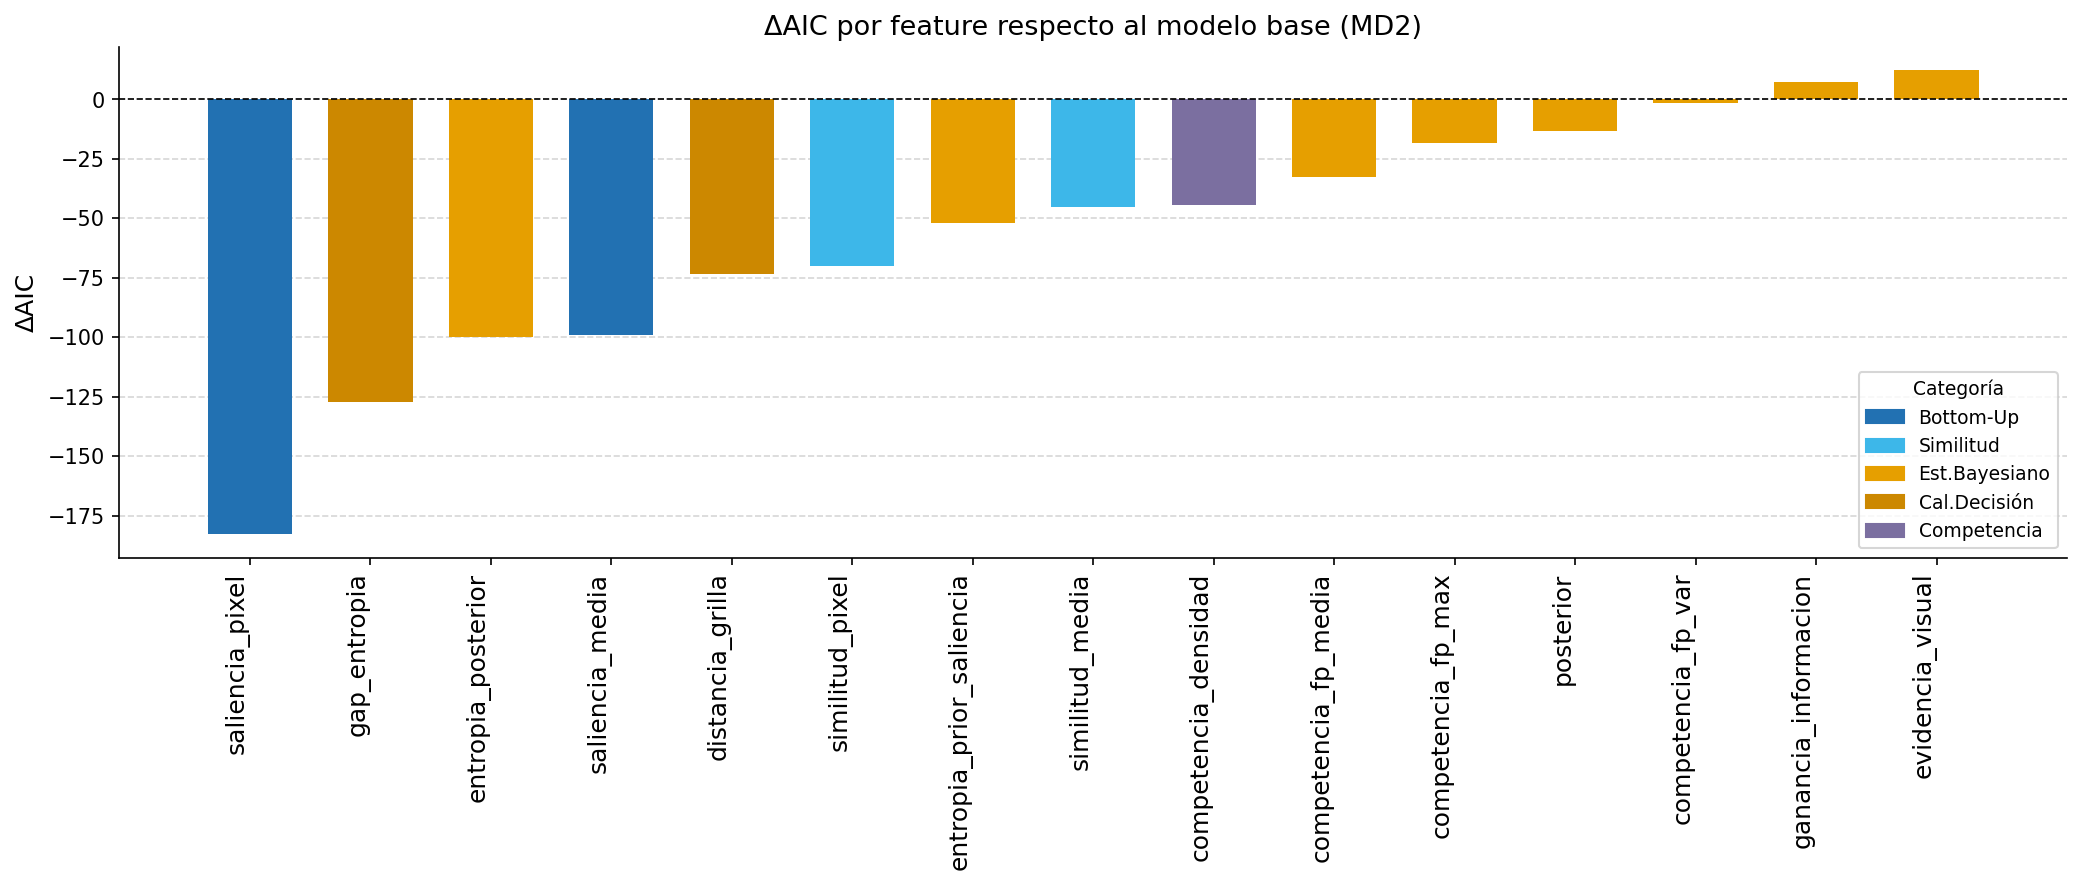
\includegraphics[width=\textwidth]{chapters/04_resultados/images/delta_aic_barras}
    \caption{$\Delta$AIC para features en escala original, coloreadas por categoría y ordenadas por valor de $\Delta$AIC.}
    \label{fig:delta_aic}
\end{figure}


% \begin{table}[H]
% \label{tab:delta_aic_base}
% \centering
% \begin{tabular}{llr}
% \toprule
% \textbf{Categoría} & \textbf{Feature} & \textbf{$\Delta$AIC} \\
% \midrule
% \multirow{3}{*}{Bottom-up} 
%   & saliencia\_pixel    & $-182{,}97$ \\
%   & saliencia\_media    & $-99{,}20$ \\
%   & saliencia\_mediana  & $-92{,}55$ \\
% \midrule
% \multirow{3}{*}{Similitud con el target} 
%   & similitud\_pixel    & $-70{,}15$ \\
%   & similitud\_media    & $-45{,}29$ \\
%   & similitud\_mediana  & $-44{,}76$ \\
% \midrule
% \multirow{6}{*}{Estado interno del proceso bayesiano} 
%   & entropia\_posterior         & $-100{,}16$ \\
%   & competencia\_ratio          & $-83{,}00$ \\
%   & ganancia\_informacion       & $7{,}43$ \\
%   & entropia\_prior\_saliencia  & $-51{,}93$ \\
%   & competencia\_fp\_media      & $-32{,}70$ \\
%   & competencia\_fp\_max        & $-18{,}45$ \\
%   & posterior                   & $-13{,}28$ \\
%   & evidencia\_visual           & $12{,}12$ \\
%   & competencia\_fp\_var        & $-1{,}77$ \\
% \midrule
% \multirow{2}{*}{Calidad de la decisión} 
%   & gap\_entropia       & $-127{,}46$ \\
%   & distancia\_grilla   & $-73{,}56$ \\
%   & distancia\_pixels   & $-73{,}56$ \\
% \midrule
% \multirow{3}{*}{Competencia entre candidatos} 
%   & competencia\_densidad       & $-44{,}67$ \\
%   & competencia\_densidad\_norm & $-44{,}67$ \\
%   & competencia\_fp\_media      & $-32{,}70$ \\
% \bottomrule
% \end{tabular}
% \caption{$\Delta$AIC para features en escala original, ordenadas por categoría y % valor de $\Delta$AIC.}
% \label{tab:delta_aic_base}
% \end{table}

\subsection{Resultados TFCE}

La significancia estadística de los efectos fue evaluada mediante TFCE sobre 
los modelos correspondientes a cada feature en escala original. De las 15 features 
evaluadas, 4 presentaron clusters espacio-temporales significativos: 
\feat{posterior}, \feat{saliencia\_media}, \feat{saliencia\_pixel} y 
\feat{similitud\_pixel}.

\begin{figure}[H]
    \centering
    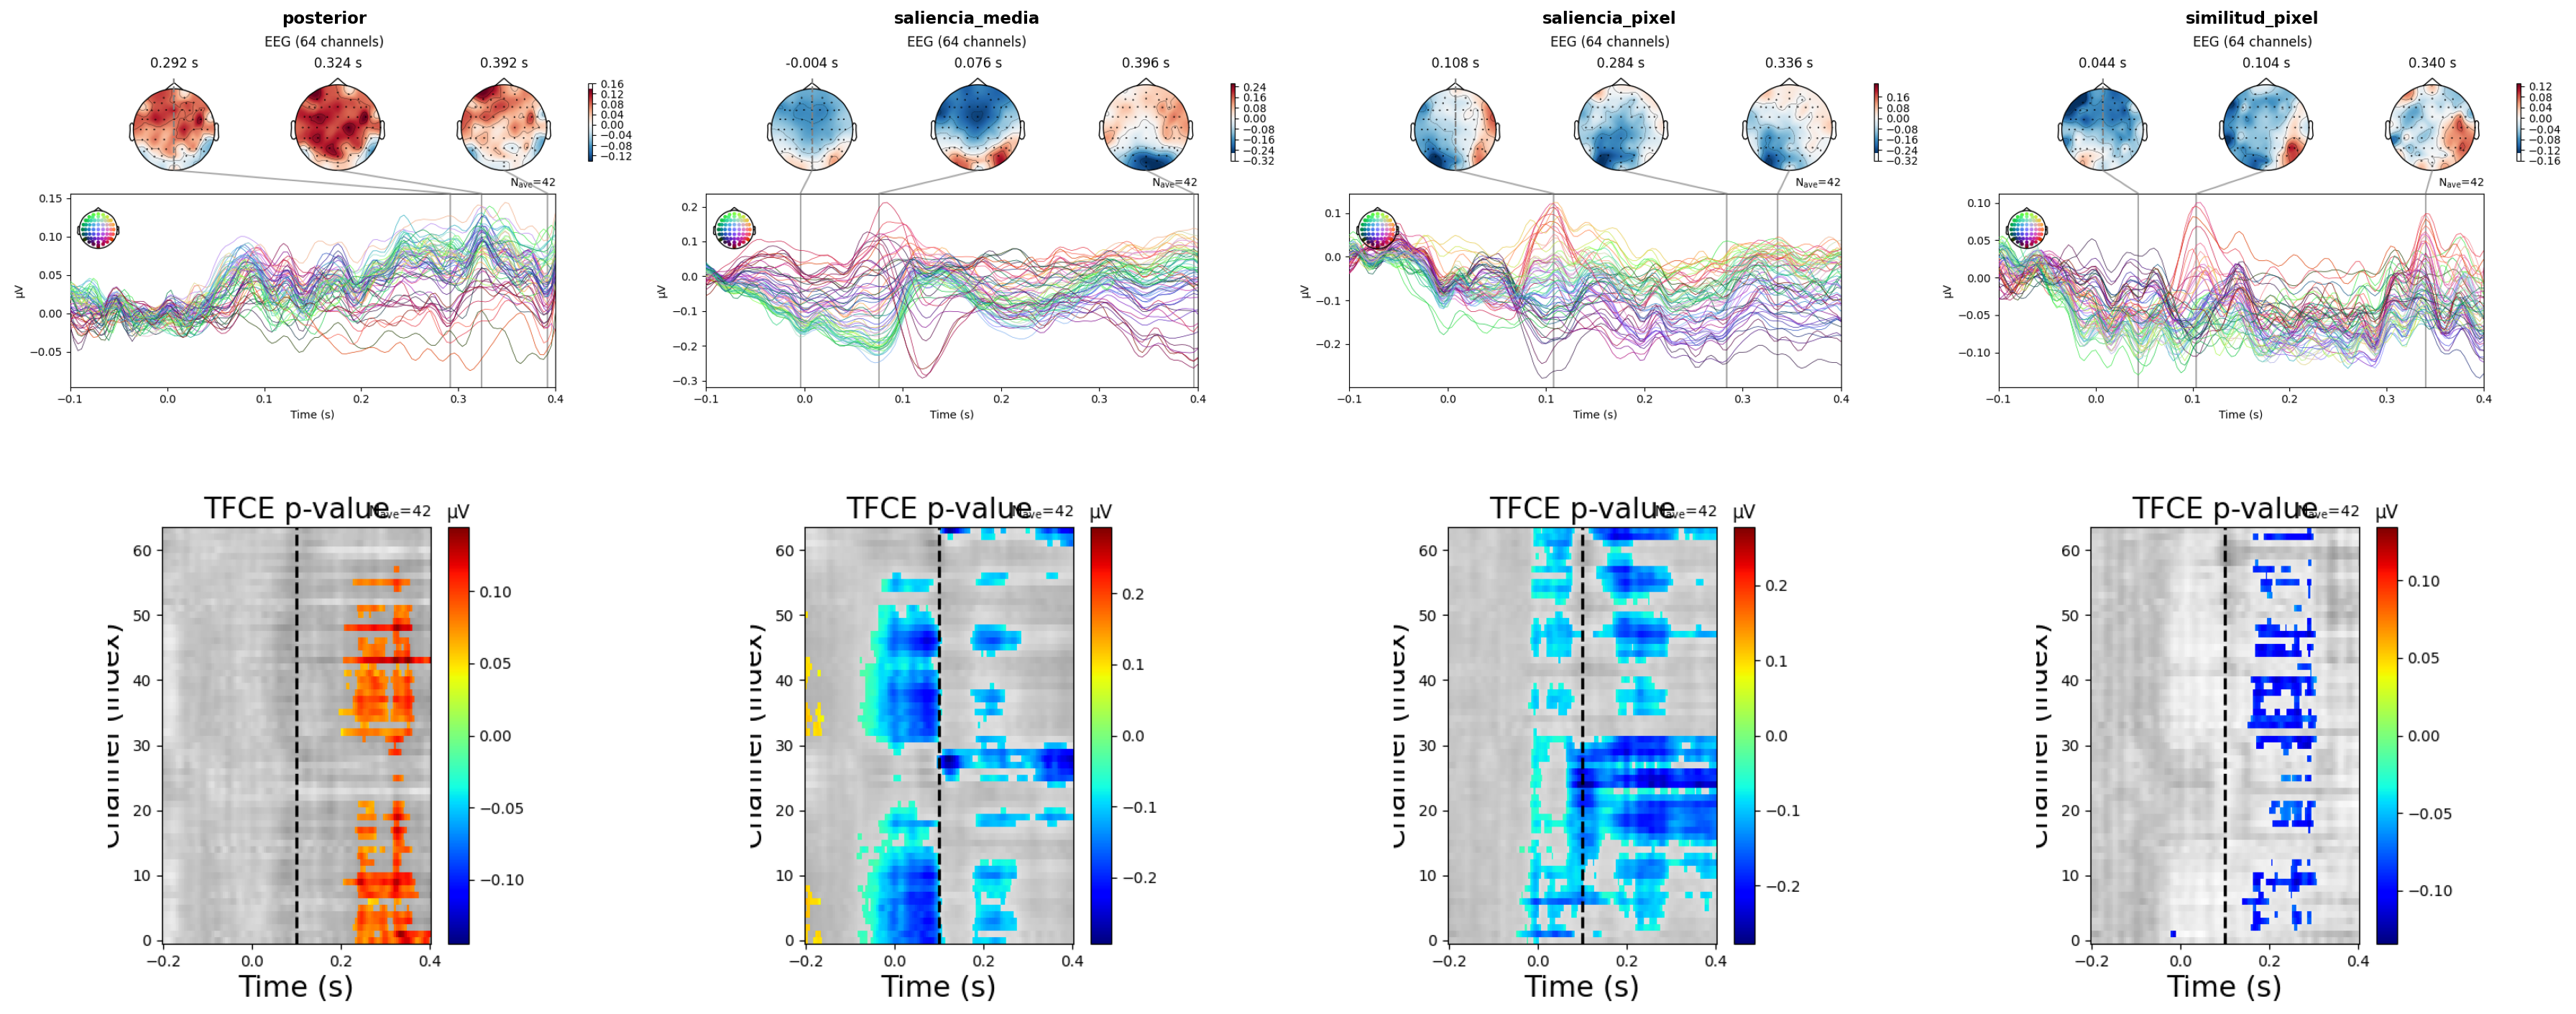
\includegraphics[width=\textwidth]{chapters/04_resultados/images/resultados_TFCE_base}
    \caption{Resultados TFCE para las features con clusters significativos en escala original: \feat{posterior}, \feat{saliencia\_media}, \feat{saliencia\_pixel} y \feat{similitud\_pixel}.}
    \label{fig:resultados_TFCE_base}
\end{figure}

La feature \feat{posterior} muestra una activación positiva que aparece alrededor de los 200 ms luego de la fijación, con distribución topográfica centro-parietal. La latencia y la distribución son consistentes con el componente P300. Una posible hipótesis es que cuando el modelo nnELM asigna alta probabilidad posterior a la celda fijada, el cerebro genera una respuesta tardía similar a la que se observa ante estímulos de relevancia para la tarea. 

Las features \feat{saliencia\_media} y \feat{saliencia\_pixel} presentan el mismo patrón: una activación negativo con un pico consistente con el componente P100. Se observan algunas diferencias entre las features: en \feat{saliencia\_media} se observa una activación de mayor amplitud y distribución fronto-central, mientras que en \feat{saliencia\_pixel} la topografía predominante es la occipital y la amplitud es menor. Una observación muy importante es que ambas features exhiben activación significativa previo al onset de la fijación; para analizarlo, en futuros trabajos se podría abordar un análisis del modelado de la señal en relación a la sacada en lugar de la fijación.

La feature \feat{similitud\_pixel} presenta una activación negativa y un patrón más complejo para analizar. Se observan latencias tempranas y tardías, con una distribución que involucra electrodos fronto-centrales y parietales.

Las 11 features restantes no presentaron clusters significativos según el 
criterio TFCE, entre ellas todas las features de calidad de la decisión 
(\feat{gap\_entropia}, \feat{distancia\_grilla}), las de competencia 
entre candidatos (\feat{competencia\_densidad}, \feat{competencia\_fp\_max}, 
\feat{competencia\_fp\_media}, \feat{competencia\_fp\_var}), el estado 
interno (\feat{entropia\_posterior}, \feat{entropia\_prior\_saliencia}, 
\feat{ganancia\_informacion}, \feat{evidencia\_visual}) y 
\feat{similitud\_media}.


